



\begin{table*}[ht]
    \centering
    \resizebox{\textwidth}{!}{%
        \setlength\tabcolsep{5pt} % Adjust column separation for better spacing
        \renewcommand{\arraystretch}{1.2} % Adjust row height for readability
        \begin{tabular}{lccccccccccc}
            \toprule
            \textbf{Model} & \textbf{Downsample Factor} & \textbf{\#Channels} & \multicolumn{3}{c}{\textbf{WebVid Test Set~\cite{bain2021frozen}}} & \multicolumn{3}{c}{\textbf{Inter4K Test Set~\cite{inter4K}}} & \multicolumn{3}{c}{\textbf{Large Motion Test Set}}\\
            \cmidrule(lr){4-6} \cmidrule(lr){7-9} \cmidrule(lr){10-12}
            & & & \textbf{PSNR ($\uparrow$)} & \textbf{SSIM ($\uparrow$)} & \textbf{LPIPS ($\downarrow$)} & \textbf{PSNR ($\uparrow$)} & \textbf{SSIM ($\uparrow$)} & \textbf{LPIPS ($\downarrow$)} & \textbf{PSNR ($\uparrow$)} & \textbf{SSIM ($\uparrow$)} & \textbf{LPIPS ($\downarrow$)} \\
            \midrule
            Open-Sora-Plan (OD VAE~\cite{chen2024odvaeomnidimensionalvideocompressor}) & 4x8x8 & 4 & 29.1646 & 0.8334 & 0.0789 & 28.6690 & 0.8381 & 0.0906 & \underline{\underline{27.5697}} & \underline{\underline{0.8045}} & 0.1065 \\
            Open-Sora (OPS VAE~\cite{opensora})& 4x8x8 & 4 & 29.3753 & 0.8284 & 0.1240 & \textbf{29.2721} & 0.8431 & 0.1316 & \textbf{27.7586} & 0.8032 & 0.1540 \\
            CV-VAE~\cite{zhao2024cv}  & 4x8x8 & 4 & 28.6795 & 0.8154 & 0.1072 & 27.7437 & 0.8124 & 0.1284 & 26.9456 & 0.7849 & 0.1411 \\
            \textbf{Video VAE w/o Joint Training (Ours)} & 4x8x8 & 4 & \underline{30.2091} & \underline{0.8656} & \underline{\underline{0.0566}} & 28.9048 & \underline{0.8543} & \underline{\underline{0.0688}} & 27.3917 & \underline{0.8078} & \underline{\underline{0.0867}}     \\
            \textbf{Video VAE (Ours)} & 4x8x8 & 4 & \textbf{30.3140} & \textbf{0.8676} & \textbf{0.0538} & \underline{\underline{28.9227}} & \textbf{0.8565} & \textbf{0.0665} & \underline{27.6236} & \textbf{0.8136} & \textbf{0.0841} \\
            \textbf{Cross-Modal VAE (Ours)} & 4x8x8 & 4 & \underline{\underline{30.1110}} & \underline{\underline{0.8608}} & \underline{0.0544} & \underline{29.0357} & \underline{\underline{0.8510}} & \underline{0.0678} & 27.1754 & 0.7999 & \underline{0.0846} \\
            \midrule
            Cosmos-Tokenizer~\cite{cosmos_token} & 4x8x8 & 16 & 31.2545 & 0.8861 & 0.1030 & 31.2002 & 0.8957 & 0.1071 & 30.1619 & 0.8675 & 0.1194 \\
            CogVideoX-VAE~\cite{yang2024cogvideox} & 4x8x8 & 16 & 32.8940 & 0.9208 & 0.0504 & 32.5122 & 0.9229 & 0.0532 & 31.0906 & 0.8978 & 0.0685 \\
            EasyAnimate-VAE~\cite{xu2024easyanimatehighperformancelongvideo} & 4x8x8 & 16 & 32.1233 & 0.9085 & 0.0405 & 31.5066 & 0.9048 & 0.0572 & 30.5213 & 0.8846 & 0.0598 \\
            CV-VAE~\cite{zhao2024cv} & 4x8x8 & 16 & 32.2766 & 0.9080 & 0.0546 & 31.6129 & 0.9060 & 0.0642 & 30.7136 & 0.8868 & 0.0726 \\
            \textbf{Video VAE w/o Joint Training (Ours)} & 4x8x8 & 16 & \underline{\underline{33.8844}} & \underline{\underline{0.9334}} & \underline{\underline{0.0344}} & \underline{\underline{32.9416}} & \underline{\underline{0.9297}} & \underline{\underline{0.0409}} & \underline{\underline{31.8471}} & \underline{\underline{0.9073}} & \underline{\underline{0.0499}} \\
            \textbf{Video VAE (Ours)} & 4x8x8 & 16 & \underline{34.1558} & \underline{0.9362} & \textbf{0.0271} & \underline{33.3184} & \underline{0.9328} & \textbf{0.0316} & \underline{32.1503} & \textbf{0.9122} & \textbf{0.0409} \\
            \textbf{Cross-Modal VAE (Ours)} & 4x8x8 & 16 & \textbf{34.5022} & \textbf{0.9365} & \underline{0.0323} & \textbf{33.5687} & \textbf{0.9347} & \underline{0.0379} & \textbf{32.2387} & \underline{0.9117} & \underline{0.0481} \\
            \bottomrule
        \end{tabular}
    }
    \caption{Quantitative comparison with state-of-the-art methods.}
    \label{tab:main}
\end{table*}





\begin{table}[ht]
    \centering
    \setlength\tabcolsep{4pt} % Increased column separation for better spacing
    \renewcommand{\arraystretch}{1} % Increased row height for readability
    \begin{tabular}{lcccc}
        \toprule
        \textbf{Model} & \textbf{\# Ch} & \textbf{PSNR ($\uparrow$)} & \textbf{SSIM ($\uparrow$)} & \textbf{LPIPS ($\downarrow$)} \\
        \midrule
        SD1.4~\cite{blattmann2023stable} & 4 & 30.2199 & 0.8974 & 0.0440 \\
        \textbf{Ours w/o JT$^*$} & 4 & 15.1001 & 0.5561 & 0.4339 \\
        \textbf{Ours} & 4 & \textbf{30.8650} & \textbf{0.9042} & \textbf{0.0397} \\
        \midrule
        SD3.5~\cite{sd35}  & 16 & \textbf{36.5208} & \textbf{0.9646} & \textbf{0.0116} \\
        \textbf{Ours w/o JT$^*$} & 16 & 9.2603 & 0.2770 & 0.6802 \\
        \textbf{Ours} & 16 & \underline{35.3437} & \underline{0.9590} & \underline{0.0167} \\
        \bottomrule
    \end{tabular}
    \caption{JT$^*$ means joint training. We evaluate image reconstruction performance w/ or w/o our joint image-video training strategy.}
    \label{tab:ablation_joint}
    \vspace{-3mm}
\end{table}



\section{Experiments}

\subsection{Experimental Setup}
\paragraph{Datasets} 
We conduct experiments on three datasets: the public Panda2M~\cite{chen2024panda} and MMTrailer~\cite{chi2024mmtrailmultimodaltrailervideo} datasets, and a private text-video dataset with over 6M pairs.
To evaluate reconstruction performance, we use three test sets: the WebVid test set, the Inter4K test set (similar to~\cite{zhao2024cv}), and a large motion test set. The WebVid test set contains 1,000 256x256, 16-frame videos from the WebVid dataset~\cite{bain2021frozen}. The Inter4K test set consists of 500 640x864, 16-frame videos from the Inter4K dataset~\cite{inter4K}.
To assess the model's ability to handle challenging motion patterns, we introduce a large motion test set. This set includes 80 videos from WebVid and 20 from Inter4K, manually selected for their complex motion dynamics.

\paragraph{Implementation Details}
We initialize our 4-channel and 16-channel latent Video VAEs from SD-1.4~\cite{rombach2022high} and SD-3.5~\cite{sd35}, respectively. For both models, we enable the video GAN loss after 50K warmup steps.
We initially train the 4-channel and 16-channel latent Video VAEs for 230K and 310K steps, respectively. Subsequently, we conduct joint image-video training, using an 8:2 video-to-image ratio to balance video and image reconstruction. For each training step, we sample 16 videos from Panda2M and our private text-video dataset, concatenating their frames into a single image batch. By masking the temporal dimension and bypassing the temporal autoencoder, we treat these images as independent static frames, allowing the model to learn from both temporal and spatial information.
The 4-channel and 16-channel latent Video VAEs undergo additional joint training for 100K and 185K steps, respectively.
For the cross-modal VAE, both models are initialized with their pre-trained weights. We train them on video-text pairs for 160K steps, enabling the model to learn the alignment between visual and textual modalities.




\subsection{Comparison with State-of-the-arts}

We compare our proposed Video VAE models with the state-of-the-art video compression models: Open-Sora-Plan~\cite{pku_yuan_lab_and_tuzhan_ai_etc_2024_10948109}, Open-Sora~\cite{opensora}, CV-VAE~\cite{zhao2024cv} on 4-channel latent models, and Cosmos-Tokenizer~\cite{cosmos_token}, CogVideoX~\cite{yang2024cogvideox}, EasyAnimate~\cite{xu2024easyanimatehighperformancelongvideo}, CV-VAE~\cite{zhao2024cv} on 16-channel models. 

\paragraph{Quantitative Evaluation}
We use PSNR, SSIM, and LPIPS~\cite{lpips} to quantitatively measure the quality of the reconstructed videos. We compare our method with baselines on our three test sets, as listed in Table~\ref{tab:main}. 
Among these, our 4-channel latent Video VAE demonstrates superior performance across most datasets and metrics. 
Specifically, our model achieves the best reconstruction quality on the WebVid test set, shown as more than 1dB improvements over baselines and a significant improvement on the LPIPS metrics, which indicates our reconstruction is both with high-fidelity and better perceptual quality. A similar conclusion can be made on the Inter4K test set. On the Large-Motion test set, our model maintains strong performance with a significant SSIM and LPIPS improvement, showcasing its robustness in handling complex motion scenarios.


For models with 16-channel latent space, our model consistently outperforms these baselines across all test sets. 
For example, on the WebVid test set, our model achieves more than 2dB in terms of PSNR, significantly higher than Cosmos-Tokenizer and CogVideoX. Moreover, our model achieves the best SSIM and LPIPS, demonstrating substantial improvements in both fidelity and perceptual quality.


In summary, our Video VAE models consistently outperform existing baselines across all test sets and metrics, highlighting their effectiveness in both low-channel (4-channel latent) and high-channel (16-channel latent) configurations.


\paragraph{Qualitative Evaluation}
We provide qualitative comparisons with the baselines in Fig.~\ref{fig:teaser}. Our method demonstrates significantly improved motion recovery, greatly reducing ghosting artifacts even in rapid motion scenarios. In contrast, Open-Sora-Plan and CV-VAE struggle to reconstruct fast-moving objects, leading to ghosting artifacts. Additionally, Open-Sora VAE introduces color reconstruction errors, as seen in the clothing of the moving figure. Increasing the latent channels to 16 improves motion reconstruction across all baselines, but noticeable detail errors remain. Our 16-channel model further mitigates these errors, resulting in more accurate detail reconstruction.
We further compare the reconstruction results with and without the cross-modal training, as shown in Fig.~\ref{fig:cross}.



\subsection{Ablation Study}



\begin{figure}[t]
\centering
\includegraphics[width=0.48\textwidth]{images/crossattn.pdf}
\caption{The effectiveness of the cross-modal learning for our video VAE. The introduction of textural information improves the detail recovery. We visualize the learned attention map using keywords of the input prompts. 
}
\label{fig:cross}
\vspace{-3mm}
\end{figure}

\paragraph{Joint Training}
We evaluate the effectiveness of our image-video joint training by comparing the performance of our 4-channel latent and 16-channel latent Video VAEs with the video-only training VAE, as well as the image VAE,  SD 1.4 and SD 3.5, respectively. The results are shown in Table~\ref{tab:main} and Table~\ref{tab:ablation_joint}. The video reconstruction comparison is conducted on the three benchmark datasets. The image reconstruction comparison is conducted on a set of 500 images with a resolution of 480x864, randomly sampled from a UHD-4K video dataset. 
During inference, we mask out the temporal autoencoder and the temporal part of the temporal-aware spatial autoencoder, ensuring that the models process the images without considering temporal information, effectively treating them as independent images.

The joint training can further boost the performance of video reconstruction, which is consistent in both the 4-channel and 16-channel experiments. 
For the image reconstruction, our 4-channel latent Video VAE slightly outperforms SD1.4, and also improves on SSIM and LPIPS, indicating better perceptual quality.

For the 16-channel VAE, while our model achieves competitive results in terms of PSNR, it falls slightly short of SD3.5. However, our model still demonstrates strong performance in terms of SSIM and LPIPS, suggesting that our joint training approach maintains high perceptual quality despite the slight drop in PSNR.

We further show the visual effectiveness of the joint image and video training in Fig~\ref{fig:joint}. Overall, these results demonstrate that our joint image-video training strategy allows the model to retain strong image reconstruction capabilities while simultaneously learning to handle video data.

\begin{figure}[t]
\centering
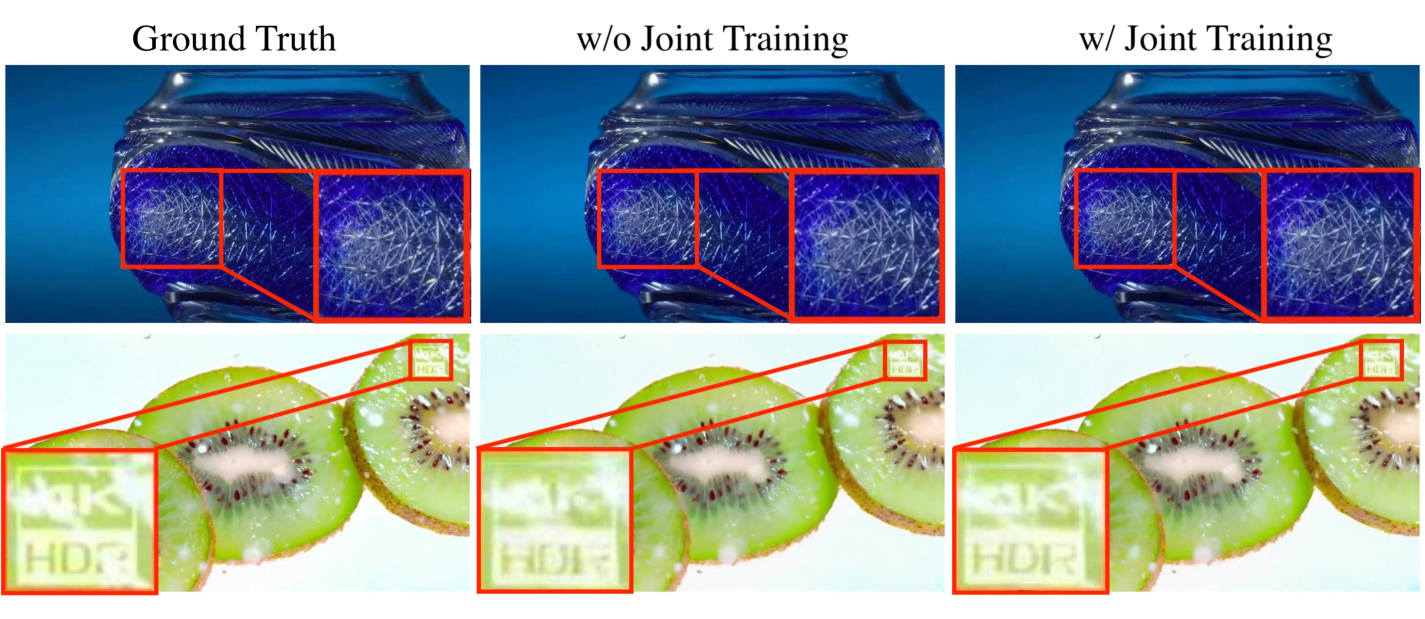
\includegraphics[width=0.5\textwidth]{images/joint_result.pdf}
\caption{The effectiveness of joint image and video training.   
}
\label{fig:joint}
\vspace{-5mm}
\end{figure}


\begin{table}[ht]
    \centering
    \setlength\tabcolsep{2pt} % Adjusted column separation for better spacing
    \renewcommand{\arraystretch}{1.2} % Adjusted row height for readability
    \begin{tabular}{lcccc}
        \toprule
        \textbf{Model} & \textbf{PSNR ($\uparrow$)} & \textbf{SSIM ($\uparrow$)} & \textbf{LPIPS ($\downarrow$)} \\
        \midrule 
        \textbf{Simultaneous } & \underline{24.0593} & \textbf{0.7315} & \underline{0.1293} \\
        \textbf{Sequential} & 23.3681 & 0.6917 & 0.1481 \\
        \textbf{Ours} & \textbf{24.6722} & \underline{0.7234} & \textbf{0.1162} \\
        \bottomrule
    \end{tabular}
    \caption{Ablation study comparing simultaneous modeling, sequential modeling, and ours on the large-motion test set.}
    \label{tab:ablation_architecture}
    \vspace{-5mm}
\end{table}


\paragraph{Architecture Variants}
We evaluate the effectiveness of different spatiotemporal compression strategies, including simultaneous spatiotemporal compression, sequential spatiotemporal compression, and our proposed solution. These architecture variants are tested on the Large-Motion Test Set to determine which model handles challenging scenarios most effectively, as shown in Table~\ref{tab:ablation_architecture}. 

\begin{table}[ht]
    \centering
    \setlength\tabcolsep{2pt} % Adjusted column separation for better spacing
    \renewcommand{\arraystretch}{1} % Adjusted row height for readability
    \begin{tabular}{lcccc}
        \toprule
        \textbf{Model / Kernel Size} & \textbf{PSNR ($\uparrow$)} & \textbf{SSIM ($\uparrow$)} & \textbf{LPIPS ($\downarrow$)}  \\
        \midrule
        \textbf{Image GAN Loss} &  \underline{31.9133} & \underline{0.9071} & \underline{0.0436}  \\
        \textbf{Video GAN Loss} & \textbf{32.0262} & \textbf{0.9089} & \textbf{0.0426} \\
        \midrule
        \textbf{TemporalConv(3, 1, 1)} & 30.3332 & 0.8898 & 0.0489 \\
        \textbf{TemporalConv(5, 1, 1)} & 30.8745 & 0.9004 & 0.0475  \\
        \textbf{TemporalConv(7, 1, 1)} & 31.2922 & \underline{0.9025} & 0.0458  \\
        \textbf{TemporalConv(5, 3, 3)} & \underline{31.3516} & 0.9011 & \underline{0.0437}  \\
        \textbf{TemporalConv(7, 3, 3)} & \textbf{31.7444} & \textbf{0.9074} & \textbf{0.0436}  \\
        \bottomrule
    \end{tabular}
    \caption{Ablation study comparing temporal-aware spatial autoencoder with image/video GAN loss, and different kernel sizes.}
    \label{tab:ablation_combined}
    \vspace{-5mm}
\end{table}



\paragraph{Component Ablation}
We perform ablation studies on several key components of our model. First, we investigate the impact of the kernel size in the temporal convolutional layer of temporal-aware spatial autoencoder. The results of this study are shown in Table \ref{tab:ablation_combined}. Additionally, we explore the significance of the loss function by comparing the performance of temporal-aware spatial autoencoder trained with either the raw image GAN loss or the video GAN loss, with the results also presented in Table \ref{tab:ablation_combined}. These ablations are conducted on a validation set comprising 98 videos, each with a resolution of 256x256 pixels and a length of 16 frames, sourced from the MMTrailer dataset.








